\documentclass[11pt,oneside]{ctexbook}
\usepackage[a4paper,margin=2.6cm]{geometry}
\usepackage[colorlinks=true,linkcolor=magenta,urlcolor=cyan,citecolor=cyan]{hyperref}
\usepackage{graphicx}
\usepackage{booktabs}
\usepackage{listings}
\usepackage{xcolor}
\usepackage[framemethod=TikZ]{mdframed}
\usepackage{xurl}
\usepackage{array}
\usepackage{tabularx}
\usepackage{float}
\usepackage{multicol}
\usepackage{etoc}
\usepackage[inline]{asymptote}

\lstset{
  basicstyle=\ttfamily\small,
  numbers=left,
  numberstyle=\tiny,
  breaklines=true,
  columns=fullflexible,
  showstringspaces=false,
  tabsize=2,
  xleftmargin=2em,
  numbersep=8pt,
}

\mdfdefinestyle{codebox}{%
  roundcorner=5pt,%
  linecolor=black!30,%
  linewidth=0.5pt,%
  backgroundcolor=gray!5,%
  innerleftmargin=0pt,%
  innerrightmargin=6pt,%
  innertopmargin=4pt,%
  innerbottommargin=4pt,%
  skipabove=6pt,%
  skipbelow=6pt,%
}
\surroundwithmdframed[style=codebox]{lstlisting}
\let\origLstInputListing\lstinputlisting
\renewcommand{\lstinputlisting}[2][]{%
  \begin{mdframed}[style=codebox]%
    \origLstInputListing[#1]{#2}%
  \end{mdframed}%
}

\title{11 分钟学会 tsqx}
\author{LeyuDame}
\date{\today}

\begin{asydef}
usepackage("amsmath");
usepackage("amssymb");
import geometry;
// recalibrate fill and filldraw for conics
void filldraw(picture pic = currentpicture, conic g, pen fillpen=defaultpen, pen drawpen=defaultpen)
    { filldraw(pic, (path) g, fillpen, drawpen); }
void fill(picture pic = currentpicture, conic g, pen p=defaultpen)
    { filldraw(pic, (path) g, p); }
pair footP(pair P, pair A, pair B) { return foot(triangle(A,B,P).VC); }
pair ortho(pair A, pair B, pair C) { return orthocentercenter(A,B,C); }
\end{asydef}

\begin{document}
\frontmatter

\begin{titlepage}
	\centering
	\vspace*{1.6cm}
	\IfFileExists{figures/fig1.pdf}{
		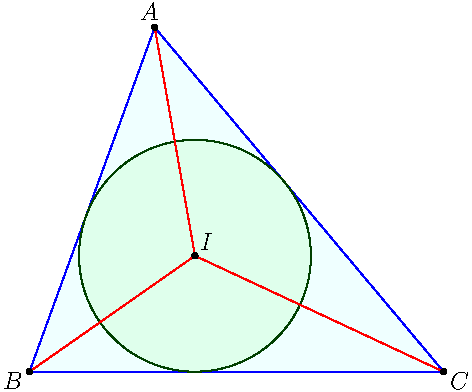
\includegraphics[width=0.48\linewidth]{figures/fig1.pdf}\par
	}{
		\fbox{\parbox{0.65\linewidth}{\centering 封面插图文件缺失: figures/fig1.pdf}}\par
	}
	\vspace{1.4cm}
	{\centering\Huge\bfseries 10 分钟学会 tsqx\par}
	\vspace{0.8em}
	{\centering\Large 一份(非常)简短的 tsqx 介绍\par}
	\vspace{1.6em}
	{\large LeyuDame\par}
	\vspace{0.5em}
	{\large \today\par}
	\vfill
\end{titlepage}

\etocsettocstyle{\begin{multicols}{2}}{\end{multicols}}
\tableofcontents
\mainmatter

\chapter*{前言}
\addcontentsline{toc}{chapter}{前言}
\section{tsqx、Asymptote、TikZ 与 \LaTeX 的关系}
如果你刚开始接触 LaTeX 排版, 很可能已经被一堆工具名字砸中了脑袋: LaTeX、TikZ、Asymptote、tsqx……它们到底是什么关系?非要学这么多吗?别慌, 它们的关系其实可以用一句话概括:
\begin{quote}
	\textbf{LaTeX} 是老板, \textbf{TikZ} 和 \textbf{Asymptote} 是两位画师, 而 \textbf{tsqx} 是专门给 Asymptote 打下手的实习生。
\end{quote}
更准确一点说: LaTeX 负责整个文档的排版(文字、公式、章节结构)；TikZ 和 Asymptote 是来自两个派系的绘图工具, 各有所长；而 tsqx 是 Asymptote 的一个速记前端——你用更简洁的语法描述几何关系, tsqx 自动帮你翻译成 Asymptote 代码。

关于 LaTeX 的基础语法知识, 相信有兴趣打开并深入阅读此文档的读者, 肯定已经具备, 在这里就不做过多展开。

下面看一下 TikZ 和 Asymptote 之间基础语法的对比——同样画一个三角形 $ABC$ 并在顶点 $A$ 作高, 两种工具的写法差距一目了然。

\medskip
\noindent\textbf{TikZ 写法（LaTeX 内部）}

TikZ 把坐标和样式全部写在一起, 和 LaTeX 正文无缝融合。语法上有点像一笔一划地吩咐画师：先指定坐标, 再声明每条线怎么画, 标签用 \texttt{node} 贴上去。

\begin{lstlisting}[language=tex]
\begin{tikzpicture}
  % 定义三个顶点坐标
  \coordinate (A) at (1, 3);
  \coordinate (B) at (0, 0);
  \coordinate (C) at (4, 0);

  % 画三角形轮廓, 填浅蓝色
  \filldraw[fill=cyan!15, draw=blue] (A) -- (B) -- (C) -- cycle;

  % 计算 A 到 BC 的垂足 D, 画高线（红色虚线）
  \coordinate (D) at ($(B)!(A)!(C)$);
  \draw[red, dashed] (A) -- (D);

  % 标注顶点标签
  \node[above]       at (A) {$A$};
  \node[below left]  at (B) {$B$};
  \node[below right] at (C) {$C$};
  \node[below]       at (D) {$D$};
\end{tikzpicture}
\end{lstlisting}

注意垂足 $D$ 需要借助 \texttt{calc} 库的 \texttt{\$(B)!(A)!(C)\$} 语法求投影点——已经算相当简洁的写法了, 但对初学者来说光这一行就要花些时间理解。

\medskip
\noindent\textbf{Asymptote 写法（独立脚本）}

Asymptote 是独立于 LaTeX 的绘图语言, 语法更接近 C++/Python。几何函数是内置的, 不需要手算坐标, 语义也更清晰——垂足就叫 \texttt{foot}, 不需要自己推投影公式。

\begin{lstlisting}[language={}]
size(6cm);
import geometry;

// 定义三个顶点（手动指定坐标）
pair A = (1, 3);
pair B = (0, 0);
pair C = (4, 0);

// 画三角形轮廓, 填浅蓝色
filldraw(A--B--C--cycle, opacity(0.15)+cyan, blue);

// 求 A 到 BC 的垂足, 画高线（红色虚线）
pair D = foot(A, B, C);
draw(A--D, red + dashed);

// 标注顶点标签
dot($A$, A, N);
dot($B$, B, SW);
dot($C$, C, SE);
dot($D$, D, S);
\end{lstlisting}

相比 TikZ, Asymptote 的代码量相近, 但几何语义更直观：\texttt{foot(A, B, C)} 直接就是$A$ 到直线 $BC$ 的垂足, 不需要记投影公式。代价是：Asymptote 是独立程序, 需要单独编译, 不能像 TikZ 那样直接写在 \texttt{.tex} 文件里（当然, 用 \texttt{asy} 环境也可以内嵌, 参考后面的章节）。

\medskip
两段代码都能画出同一张图。选择哪个？简单规则是：\textbf{图简单、需要和正文紧密配合, 用 TikZ；图复杂、需要大量几何构造, 用 Asymptote（加上 tsqx）}。

\section{关于 Evan Chen 与 tsqx 项目}

Evan Chen\footnote{中文名陈谊廷，个人网站: \url{https://web.evanchen.cc/}} 是美国数学竞赛领域的知名人物, 曾是国际数学奥林匹克(IMO)的金牌得主, 后来还担任美国数学奥林匹克团队的领队和教练。他在竞赛几何方面的造诣非常深厚, 也是一位出色的教育者和作者。Evan Chen 的《Euclidean Geometry in Mathematical Olympiads》被誉为竞赛几何的圣经, 书中系统地总结了各种经典几何构造和技巧, 深受全球竞赛选手和教练的喜爱。

\textbf{tsqx} 正是 Evan Chen 为解决竞赛几何作图的实际痛点而开发的项目。在教学和出题过程中, 他意识到即使是经验丰富的使用者, 用 Asymptote 画一套完整的竞赛题图也要花不少时间——大量的代码都是重复的坐标定义和样板声明。基于这个观察, tsqx 应运而生: 提供一层更接近竞赛几何语言的前端, 让使用者用自然的数学语言描述几何关系, 后端自动翻译成完整的 Asymptote 代码。

tsqx 的设计哲学是\textbf{简洁而不失灵活}——它不试图成为一个全功能的绘图语言, 而是大幅降低竞赛几何的常见构造的表达成本, 同时保留了与 Asymptote 无缝衔接的能力。这使得 tsqx 成为了出题者、讲义编写者的得力助手：一个下午需要画十几道题时, 用 tsqx 能节省大量重复劳动, 而且生成的代码易于版本管理和协作。

\section{它们分别做什么}
\begin{tabularx}{0.94\linewidth}{@{}>{\bfseries}p{0.20\linewidth}X@{}}
	\toprule
	工具        & 角色                                         \\
	\midrule
	TikZ      & LaTeX 内部绘图语言, 和正文融合紧密, 但复杂几何代码会较长。         \\
	Asymptote & 专门绘图语言, 语义清晰, 几何与竞赛图形表达力强。                 \\
	tsqx      & Asymptote 的几何预处理层, 用更短语法写图, 再转成 Asymptote。 \\
	\bottomrule
\end{tabularx}

\vspace{1cm}

你可能会问: \textit{我直接学 Asymptote 不就好了, 为什么还要多一个 tsqx?}这个问题问得很好。原因是: 竞赛几何里经常需要构造垂足、内心、交点等, 这些在 Asymptote 里要写好几行, 而在 tsqx 里往往一句话就搞定了。当一个下午要画十几道题的图时, 这个效率差距就非常明显了。

\section{与主文档和 PDF 的关系}
典型流程是: \texttt{.tsqx -> .asy -> .pdf -> .tex}。
其中图形最终都以 PDF 形式进入主文档(当然, Asymptote 也可以以其他方式导出)。整个链条的每一步都有对应的工具负责, 你只需要站在最上游写 tsqx, 剩下的交给工具链搞定。当然, 熟悉之后也可以跳过 tsqx 直接写 Asymptote——tsqx 不是枷锁, 只是一块起跳板。

\section{两种插图方式}
既然 Asymptote 代码最终都要变成图, 有两种路径可以走:
\begin{enumerate}
	\item \textbf{内嵌方式: }在主文档中直接写 \texttt{\textbackslash begin\{asy\}...\textbackslash end\{asy\}}, 编译时 LaTeX 会自动调用 Asymptote 出图。好处是图和文档在一起, 版本管理方便；坏处是编译链要跑三遍, 稍微繁琐一点。
	\item \textbf{外部方式: }先把 \texttt{.asy} 单独编译成 PDF, 再用 \texttt{\textbackslash includegraphics} 插入主文档。好处是流程透明、编译快；坏处是图和文档分离, 需要自己管好文件。
\end{enumerate}
初学者建议从第二种方式起步——先让图能画出来, 再考虑怎么嵌进文档。等你对整个工具链熟悉了, 再试试内嵌方式。

\section{内嵌 asy 的编译链}
当图形直接写在 \texttt{\textbackslash begin\{asy\}...\textbackslash end\{asy\}} 中时,
推荐编译顺序是
\begin{center}
	\texttt{XeLaTeX -> asy -> XeLaTeX}
\end{center}

听起来有点绕?其实逻辑很清晰: 第一遍 XeLaTeX 先把 \texttt{asy} 环境导出成临时 \texttt{.asy} 文件；接着 Asymptote 读取这些文件并渲染成 PDF；最后第二遍 XeLaTeX 把图回填到文档里。就像拍照要先打底稿、再冲印、再装裱——少了哪一步都不行。

如果手动操作嫌麻烦, 本仓库的 \texttt{examples/.latexmkrc} 已经把这条链全部封装好了, 直接执行

\begin{center}
	\texttt{latexmk -pdfxe tsqx\_example.tex}
\end{center}
一条命令走完全程, 等它跑完就行。

\section{顺带谈一下与 GeoGebra 的关系}
GeoGebra 是很多人入门几何作图的第一站——鼠标点一点, 图就出来了, 还能拖着玩, 非常直观。那为什么还要费事学 tsqx?

两个工具面向的场景不同: GeoGebra 适合\textbf{交互探索}, 可以拖点、动态演示；tsqx/Asymptote 则更适合\textbf{生产讲义}, 代码可以版本管理、可以复现、可以批量修改样式。一旦讲义里有几十道题的图, GeoGebra 的文件堆起来难以维护, 而文本文件(配合 Git)就方便多了。

GeoGebra 倒是可以导出 Asymptote 代码——但不客气地说, 导出来的代码通常很长、很丑、很难读懂, 大多数情况下还需要大量人工整理。所以结论是: 用 GeoGebra 探索构造, 用 tsqx 落笔成图；两者互补, 不是竞争关系。

\chapter{下载与配置 tsqx}
\section{为什么要先配置好环境}
可能有人会有个奇怪的疑问: \textit{为什么要专门花时间配环境, 而不是直接学语法?}

答案是: tsqx 本质上是个命令行工具，得先把环境配好、命令跑通，后面画图才会顺。就像学骑车，先把车调好再上路，不然再怎么练也使不上劲。

tsqx 值得你花这点时间配置, 理由有三:
\begin{enumerate}
	\item \textbf{语法极短}, 尤其适合竞赛几何常用构造(如 \texttt{foot}、\texttt{incenter}、\texttt{extension}), 写起来比原生 Asymptote 快得多
	\item \textbf{与 Asymptote 无缝衔接}: 先用 tsqx 快速搭骨架, 需要精细调整时再切换到底层 Asymptote
	\item \textbf{文本格式, Git 友好}: 讲义和题解的图的源码可以一起进版本管理, 而不是一堆神秘的二进制文件
\end{enumerate}

\section{安装 tsqx}
tsqx 是一个 Python 包\footnote{tsqx 的 GitHub 仓库地址: \url{https://github.com/vEnhance/tsqx}}, 安装方式非常简单:
\begin{lstlisting}[language=bash]
pip install tsqx
\end{lstlisting}

如果一切顺利, 安装完成后就能立刻在终端里用 \texttt{tsqx} 命令了。然而, 现实往往没有这么顺利。如果你的机器上同时有 Conda、pyenv、系统自带 Python, 或者同时存在 \texttt{python3} 和 \texttt{python}……那你很可能会遭遇明明装了, 但 \texttt{tsqx} 命令找不到的经典困境。原因是: 你的 \texttt{pip} 和运行时的 \texttt{python} 可能不是同一套环境。最稳妥的检查方式是逐条执行:
\begin{lstlisting}[language=bash]
which python
which pip
which tsqx
tsqx --help
\end{lstlisting}
如果 \texttt{which tsqx} 有输出, 并且 \texttt{tsqx --help} 能打印出帮助信息, 就说明安装成功了。如果 \texttt{tsqx} 仍然找不到, 试试 \texttt{pip3 install tsqx} 或者 \texttt{python -m tsqx --help}, 通常能绕过路径问题。

\section{安装 Asymptote}
tsqx 的输出是 Asymptote 代码, 而 Asymptote 代码还需要 Asymptote 本体才能变成图。这是两件独立的事: tsqx 负责翻译, Asymptote 负责渲染。不同操作系统上的安装方式如下:
\begin{itemize}
	\item \textbf{macOS}: 推荐用 Homebrew: \texttt{brew install asymptote}
	\item \textbf{Linux}(Debian/Ubuntu): \texttt{sudo apt install asymptote}
	\item \textbf{Windows}: 从 Asymptote 官网下载安装包, 或通过 TeX Live 附带安装
	\item \textbf{TeX Live / MiKTeX 用户}: Asymptote 通常随发行版一起安装, 直接在终端试试 \texttt{asy --version}
\end{itemize}

安装完成后, 运行 \texttt{asy --version} 能看到版本号就说明成功了。如果版本低于 2.69, 建议更新——旧版本 Asymptote 偶尔会对某些语法报错, 让你误以为是自己写错了, 其实是版本的锅。

\section{VS Code 扩展与命令路径}
如果你用 VS Code 写 tsqx, 可以安装专用扩展(在插件市场里搜索 \texttt{tsqx-compiler}\footnote{扩展地址: \url{https://marketplace.visualstudio.com/items?itemName=LYDT.tsqx-compiler}}), 实现一键将 \texttt{.tsqx} 文件编译并预览成 PDF 图。

推荐把扩展的 tsqx 命令路径指向稳定的全局环境, 或项目内脚本(如 \texttt{./bin/tsqx}), 避免 Python 环境漂移导致命令找不到。如果你用 Conda 管理环境, 记得在扩展配置里写清楚完整的可执行文件路径(如 \texttt{/Users/yourname/miniconda3/envs/myenv/bin/tsqx}), 而不要只写 \texttt{tsqx}——否则 VS Code 启动时找不到那个 Conda 环境, 你会花不少时间调试这个问题。

对新手来说, 这个扩展最大的价值是: 把改一行 tsqx、立刻看到新图的迭代循环压缩到几秒钟, 让你专注在几何构造本身, 而不是在终端里反复敲命令。

值得一提的是，如果你对于在 VS Code 当中使用 LaTeX Workshop 来编译 LaTeX 很熟悉的话，那么这个插件就相当于是 tsqx 文件的编译器。事实上，它具有类似于 LaTeX Workshop 一样的自动实时编译功能。

\section{LaTeX 文档如何配合}
配好环境之后, 来说说怎么把图塞进文档。有两条路线:

\textbf{路线一(推荐初学者): 稳妥的手工流程。}先用 tsqx 把 \texttt{.tsqx} 转成 \texttt{.asy}, 再用 Asymptote 编译成 PDF, 最后用 \texttt{\textbackslash includegraphics} 插图。虽然步骤多一点, 但每一步都很清晰, 出了问题也好定位。比如说, 如果 PDF 图不对了, 你就知道是 Asymptote 的问题；如果 \texttt{.asy} 文件里代码不对了, 就知道是 tsqx 的问题。

你可以直接打开一份 tsqx 文件，然后使用 VSCode 扩展 \texttt{tsqx-compiler} 进行编译，或者也可以在终端执行以下命令。

\begin{lstlisting}[language=bash]
tsqx -p < figures/fig3.tsqx > figures/fig3.asy
asy -f pdf -o figures/fig3 figures/fig3.asy
\end{lstlisting}

\textbf{路线二(进阶): 内嵌 asy 的自动化流程。}在主文档里直接写 Asymptote 代码, 使用本项目附带的 \texttt{latexmk} 配置自动驱动编译链。更优雅, 但编译时间稍长, 调试也需要一点耐心。

建议先走路线一, 等你对整个流程熟悉了, 再尝试路线二。

\chapter{tsqx 基本语法}
\section{最小例子}
先别急着看语法规则, 直接上手一个最简单的例子。下面这段 tsqx 代码画了一个三角形 $ABC$ 和它的内心 $I$:
\begin{lstlisting}[language={}]
# tsqx
A = dir 110
B = dir 210
C = dir 330
I 45 = incenter A B C
A--B--C--cycle / 0.12 lightcyan / blue
\end{lstlisting}

就这几行。没有分号, 没有 \texttt{pair}, 没有括号, 也没有 \texttt{opacity(...)+}。生成的图形如下:
\begin{center}
	\begin{asy}
		size(6cm);
		pair A = dir(110);
		pair B = dir(210);
		pair C = dir(330);
		pair I = incenter(A, B, C);
		filldraw(A--B--C--cycle, opacity(0.12)+lightcyan, blue);
		dot("$A$", A, dir(A));
		dot("$B$", B, dir(B));
		dot("$C$", C, dir(C));
		dot("$I$", I, dir(45));
	\end{asy}
\end{center}

tsqx 会把它翻译成完整的 Asymptote 代码(核心部分如下):
\begin{lstlisting}[language={}]
pair A = dir(110);
pair B = dir(210);
pair C = dir(330);
pair I = incenter(A, B, C);
filldraw(A--B--C--cycle, opacity(0.12)+lightcyan, blue);
\end{lstlisting}
翻译前后的语句一一对应——tsqx 的写法只是少了很多重复的样板。如果你觉得 Asymptote 版本也没复杂多少, 等你一次性需要定义十几个点的时候, 就能明显感受到差距了。

\section{tsqx 的基本思想}
有些同学一看到新工具就会问: \textit{这又是一门新语言, 我要重新学吗?}

好消息: 不用。tsqx 的核心不是重新发明一门完整绘图语言, 而是给 Asymptote 常见的几何操作加一层更短、更接近自然语言的写法。你可以把它理解为竞赛几何常用语句的速记层:
\begin{enumerate}
	\item \textbf{几何对象直接生成}: 点、线、圆和交点, 通常都能用一句话定义, 不需要手写坐标计算
	\item \textbf{画图和着色命令简短}: 改个颜色不需要改三处地方, 适合快速试图
	\item \textbf{最终落到 Asymptote}: tsqx 满足不了需求时, 直接在生成的 \texttt{.asy} 文件里手动补充代码即可
\end{enumerate}
换句话说: tsqx 让你用更少的字来表达我要画什么, 至于怎么画, 留给 Asymptote 去操心。

\section{点、对象与赋值}
tsqx 里, 点(以及其他几何对象)的定义方式非常直白——几乎就是在写数学语言:
\begin{lstlisting}[language={}]
A = dir 110
D = foot A B C
E = midpoint A--B
F = extension A D C E
\end{lstlisting}
逐句解读:
\begin{enumerate}
	\item \texttt{dir 110}: 在单位圆上取一个方向角为 $110^\circ$ 的点。\texttt{dir} 是竞赛几何标准玩法, 用来快速铺好三角形的三个顶点, 不用自己算坐标
	\item \texttt{foot A B C}: 点 $A$ 到直线 $BC$ 的垂足——\textbf{注意}参数顺序: 先写要作垂线的那个点, 再写垂足所在的直线(两点确定)
	\item \texttt{midpoint A--B}: 线段 $AB$ 的中点；这里用 \texttt{A--B}(两个短横线), 和后面画路径的写法保持一致
	\item \texttt{extension A D C E}: 直线 $AD$ 与直线 $CE$ 的交点——参数顺序是第一条直线两点, 第二条直线两点
\end{enumerate}
等号右边的函数名几乎都是英文直读, 不需要死记, 多写几次自然就记住了。

\section{初始化三角形}
竞赛几何题的开场白几乎都是设 $\triangle ABC$ 是一个三角形。tsqx 为此提供了一条快捷命令:
\begin{lstlisting}[language={}]
~triangle A B C
\end{lstlisting}

这一行会自动在单位圆上取三个合适的点作为 $A$、$B$、$C$, 生成一个不太丑、不太特殊的三角形, 并设置好画图尺寸。你完全不需要关心具体数值, 直接在后面写构造就行。

\textbf{等价写法: }\texttt{\~{}triangle A B C} 实际上是以下三行的简写——Evan Chen 预设了三个固定方向角, 使三角形形状匀称、不过于特殊:
\begin{lstlisting}[language={}]
A = dir 110
B = dir 210
C = dir 330
\end{lstlisting}
如果你想要一个形状不同的三角形, 只需把这三行里的角度改成自己想要的值即可。\texttt{dir} 函数在单位圆上取对应方向角的点, 三个角度分别取 $110^\circ$、$210^\circ$、$330^\circ$ 可以让三角形既不等腰也不直角, 是竞赛作图的常用默认值。

开头的波浪号 \texttt{\~{}} 是 tsqx 里的宏前缀, 表示这条语句会展开成一段预设的 Asymptote 代码, 而不仅仅是定义一个点。换句话说, 它帮你写了一大段初始化代码。对初学者来说, \texttt{\~{}triangle} 的最大价值是: \textbf{跳过如何摆好三个点这个问题, 直接进入画什么构造的思考}。等你对 tsqx 熟悉之后, 当然也可以手动改成自己喜欢的点坐标。

以下是 \texttt{\~{}triangle A B C} 生成的三角形效果:
\begin{center}
	\begin{asy}
		size(5cm);
		pair A = dir(110);
		pair B = dir(210);
		pair C = dir(330);
		filldraw(A--B--C--cycle, opacity(0.10)+lightcyan, blue);
		dot("$A$", A, dir(A));
		dot("$B$", B, dir(B));
		dot("$C$", C, dir(C));
	\end{asy}
\end{center}

\section{标签方向与命名}
标签方向是初学者最容易忽略的细节——一旦忘记指定, 标签就容易压到图的线段上, 看起来一团糟。tsqx 通过在变量名后面紧跟一个数字来指定标签方向角:
\begin{lstlisting}[language={}]
I 45 = incenter A B C
P' 90 = extension A B C D
\end{lstlisting}

\texttt{I 45 = ...} 里的 \texttt{45} 表示标签放置的方向(以度为单位), 对应 Asymptote 里的 \texttt{dir(45)}, 即右上方。如果不指定方向, tsqx 默认会用 \texttt{dir(point)} 自动计算——对于 \texttt{dir(110)} 这类在单位圆上的点, 自动方向通常不会太差；但对于内心、垂心这种藏在三角形内部的点, 还是手动指定比较保险。

至于变量名里的撇号(\texttt{P'}): 在数学里很常见, 在 Asymptote(本质是 C++ 语法)里却是不合法的变量名。tsqx 会自动把 \texttt{P'} 转成 \texttt{P\_prime}, 你不需要操心。类似地, \texttt{A1} 会保持原样, 只要不是 Asymptote 的保留字就问题不大。

\section{路径、描边与填色}
定义好点之后, 就该告诉 tsqx 把哪些东西画出来, 以及用什么颜色。tsqx 用斜杠 \texttt{/} 来分隔画什么和怎么画:
\begin{lstlisting}[language={}]
A--B--C--cycle / 0.12 lightcyan / blue
incircle A B C / 0.15 lightgreen / darkgreen
A--D / red
B--F dashed blue
\end{lstlisting}

规则很简单:
\begin{enumerate}
	\item \textbf{第一个 \texttt{/} 之前}: 几何对象或路径(画什么)
	\item \textbf{第一个 \texttt{/} 之后、第二个 \texttt{/} 之前}: 填充样式, 通常是透明度 + 颜色, 例如 \texttt{0.12 lightcyan} 表示 12\% 不透明度的浅青色
	\item \textbf{第二个 \texttt{/} 之后}: 描边颜色
\end{enumerate}

如果只需要描边(不填色), 可以省略所有斜杠, 直接把线型和颜色跟在路径后面, 例如 \texttt{B--F dashed blue} 表示蓝色虚线。如果连颜色都不写, 就用黑色默认描边。

\textbf{小提示: }tsqx 支持所有 Asymptote 内置的颜色名, 常用的有 \texttt{red}、\texttt{blue}、\texttt{green}、\texttt{gray}、\texttt{lightcyan}、\texttt{lightyellow} 等。需要更精确的颜色时, 可以在生成的 \texttt{.asy} 文件里手动换成 \texttt{rgb(r,g,b)} 形式。

\section{一组常见命令}
下面是竞赛几何最常用的 tsqx 命令汇总。建议先大致扫一眼, 有个印象；等真正用到时再回来查这张表。

\vspace{0.5cm}

\begin{tabularx}{0.94\linewidth}{@{}>{\ttfamily}p{0.34\linewidth}X@{}}
	\toprule
	tsqx 写法                         & 说明                   \\
	\midrule
	\textnormal{\~{}triangle A B C} & 生成常用初始三角形点位          \\
	foot P A B                      & 点 $P$ 到直线 $AB$ 的垂足   \\
	incenter A B C                  & 三角形 $ABC$ 的内心        \\
	orthocenter A B C               & 三角形 $ABC$ 的垂心        \\
	midpoint A--B                   & 线段 $AB$ 的中点          \\
	extension A B C D               & 直线 $AB$ 与直线 $CD$ 的交点 \\
	circumcircle A B C              & 三角形 $ABC$ 的外接圆       \\
	incircle A B C                  & 三角形 $ABC$ 的内切圆       \\
	A--B--C--cycle                  & 路径(多边形轮廓)            \\
	\bottomrule
\end{tabularx}

\vspace{0.5cm}

还有一些不太常见但偶尔用得到的: \texttt{CP O A}(以 $O$ 为圆心、过 $A$ 的圆)、\texttt{IP c1 c2}(两个圆的交点之一)、\texttt{OP c1 c2}(另一个交点)等。完整列表可以在 tsqx 的 Wiki 文档\footnote{\url{https://github.com/vEnhance/tsqx/wiki/Documentation}}中找到。

\section{再次回顾 tsqx 和 Asymptote 的关系}
理解了前面几节, 你其实已经掌握了 tsqx 的主要语法。再来看一个稍完整的例子, 同时体会一下 tsqx 和 Asymptote 之间的对应关系:
\begin{lstlisting}[language={}]
~triangle A B C
D = foot A B C
E = midpoint A--B
F = extension A D C E

A--B--C--cycle / 0.2 lightblue / black
A--D
C--E
B--F dashed blue
\end{lstlisting}

这段代码画了三角形 $ABC$, 以及: $A$ 到 $BC$ 的垂足 $D$；$AB$ 的中点 $E$；直线 $AD$ 与 $CE$ 的交点 $F$；三角形填上浅蓝色, 三条辅助线中 $BF$ 是虚线。

它对应的 Asymptote 核心结构就是先定义点, 再 \texttt{draw}/\texttt{filldraw}——和 tsqx 的语句完全对应, 只是写法更繁琐。如果你想验证 tsqx 翻译是否正确, 可以运行 \texttt{tsqx -p < yourfile.tsqx} 查看生成的 Asymptote 代码, 对照研究。

也正因为这种清晰的对应关系, tsqx 的学习曲线很平缓: 先用 tsqx 快速表达几何关系, 遇到 tsqx 解决不了的需求时, 再直接修改生成的 Asymptote 代码——两者之间翻墙的成本很低。

\chapter{实战篇: 三个例子}
\section{示例 1: 内心与内切圆}
内心是竞赛几何最经典的心之一, 几乎每本几何书的第一章都会遇到它。我们就用这个场景来热身: 画出三角形 $ABC$, 找到内心 $I$, 画出内切圆, 并连接三条角平分线。

\subsection{原始 tsqx 源码}
\lstinputlisting[language={}]{figures/fig1.tsqx}

只有寥寥几行: 三个顶点用 \texttt{dir} 在单位圆上取好, \texttt{incenter} 一句话搞定内心, \texttt{I 45} 把标签放在右上方, 最后几行分别填色三角形和内切圆, 再画三条红色连线。就是这么直白。

\subsection{内嵌 Asymptote 代码与成图}
\begin{center}
	\begin{asy}
		size(8cm);

		//  基础三角形 + 内心 + 内切圆
		pair A = dir(110);
		pair B = dir(210);
		pair C = dir(330);
		pair I = incenter(A, B, C);

		filldraw(A--B--C--cycle, opacity(0.12)+lightcyan, blue);
		filldraw(incircle(A, B, C), opacity(0.15)+lightgreen, darkgreen);
		draw(A--I, red);
		draw(B--I, red);
		draw(C--I, red);

		dot("$A$", A, dir(A));
		dot("$B$", B, dir(B));
		dot("$C$", C, dir(C));
		dot("$I$", I, dir(45));

		/* --------------------------------+
		| tsqx: by Evan Chen and CJ Quines |
		| https://github.com/vEnhance/tsqx |
		+----------------------------------+
		# 基础三角形 + 内心 + 内切圆
		A = dir 110
		B = dir 210
		C = dir 330
		I 45 = incenter A B C

		A--B--C--cycle / 0.12 lightcyan / blue
		incircle A B C / 0.15 lightgreen / darkgreen
		A--I / red
		B--I / red
		C--I / red
		*/
	\end{asy}
\end{center}

注意图里三条红线汇聚于内心 $I$——这正是内心的定义: 三角形三条角平分线的交点, 同时也是内切圆的圆心。tsqx 把这些几何关系用几行代码就表达清楚了, 而背后对应的 Asymptote 代码里那些 \texttt{pair}、\texttt{filldraw}、\texttt{dot}, 全部是自动生成的, 你完全不需要手写。

\section{示例 2: 垂心与垂足三角形}
如果说内心是竞赛几何的开胃小菜, 那垂心就是主菜了——与它相关的性质多如牛毛, 垂足三角形更是各种反射、共圆性质的温床。这个例子稍微复杂一点: 画三角形 $ABC$、垂心 $H$、垂足三角形 $DEF$, 以及三条高线。
\subsection{原始 tsqx 源码}
\lstinputlisting[language={}]{figures/fig2.tsqx}

留意 \texttt{foot H B C}: 意思是点 $H$ 到直线 $BC$ 的垂足, 得到高的垂足 $D$。类似地, \texttt{foot H C A} 和 \texttt{foot H A B} 分别得到另两个垂足。如果手写 Asymptote, 这三行各自需要用 \texttt{foot(triangle(B,C,H).VC)} 这样的表达式——不仅长, 还容易记混参数顺序。这时候 tsqx 的简洁性就非常突出了。

\subsection{内嵌 Asymptote 代码与成图}
\begin{center}
	\begin{asy}
		size(8cm);

		pair A = dir(95);
		pair B = dir(215);
		pair C = dir(330);
		pair H = ortho(A, B, C);
		pair D = footP(H, B, C);
		pair E = footP(H, C, A);
		pair F = footP(H, A, B);

		filldraw(A--B--C--cycle, opacity(0.08)+lightyellow, blue);
		filldraw(D--E--F--cycle, opacity(0.15)+lightcyan, red);
		draw(A--D, gray);
		draw(B--E, gray);
		draw(C--F, gray);

		dot("$A$", A, dir(A));
		dot("$B$", B, dir(B));
		dot("$C$", C, dir(C));
		dot("$H$", H, dir(H));
		dot("$D$", D, dir(D));
		dot("$E$", E, dir(E));
		dot("$F$", F, dir(F));

		/* --------------------------------+
		| tsqx: by Evan Chen and CJ Quines |
		| https://github.com/vEnhance/tsqx |
		+----------------------------------+
		# 垂心与垂足三角形
		A = dir 95
		B = dir 215
		C = dir 330
		H = orthocenter A B C
		D = foot H B C
		E = foot H C A
		F = foot H A B

		A--B--C--cycle / 0.08 lightyellow / blue
		D--E--F--cycle / 0.15 lightcyan / red
		A--D / gray
		B--E / gray
		C--F / gray
		*/
	\end{asy}
\end{center}

从图中可以清楚地看到: 三条高线(灰色)交于垂心 $H$, 垂足三角形 $DEF$(浅青色)镶嵌在原三角形内部。事实上, $H$ 是 $\triangle DEF$ 的内心——这是一个经典结论, 你现在不需要手算任何坐标就把这张图画出来了。

\section{示例 3: 外部 PDF 插图}
前两个例子用的都是内嵌 asy方式——图的代码直接写在 \texttt{.tex} 文件里, 编译时自动生成。这个例子演示另一条路线: 先用 tsqx 把 \texttt{.tsqx} 转成 \texttt{.asy}, 再手动编译成 PDF, 最后用 \texttt{\textbackslash includegraphics} 插入主文档。这条路线在需要批量编译图形、或希望图和文档相互独立时特别实用。

\subsection{原始 tsqx 源码}
\lstinputlisting[language={}]{figures/fig3.tsqx}

这个例子的 tsqx 代码稍微进阶一点: \texttt{CP L I} 表示以 $L$ 为圆心、以 $LI$ 为半径的圆；\texttt{(2*L-I)} 是直接嵌入的 Asymptote 表达式——tsqx 支持在定义里写任意 Asymptote 表达式, 遇到没有内置函数覆盖的构造时, 这个特性非常好用。

\subsection{对应 Asymptote 源码}
\lstinputlisting[language={}]{figures/fig3.asy}

对比一下 tsqx 源码(约 10 行)和 Asymptote 源码(40 多行), 就能直观感受到 tsqx 帮你省了多少字——那些 \texttt{pair ... = ...;}、\texttt{dot(..., ..., dir(...))}, 全部是自动生成的。

\subsection{先编译 ASY, 再插图}
\begin{lstlisting}[language=bash]
asy -f pdf -o figures/fig3 figures/fig3.asy
\end{lstlisting}

\IfFileExists{figures/fig3.pdf}{
	\begin{center}
		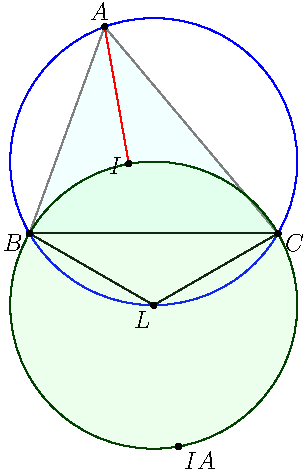
\includegraphics[width=0.3\linewidth]{figures/fig3.pdf}
	\end{center}
}{
	\textit{尚未检测到 figures/fig3.pdf。请先执行上面的 asy 命令。}
}

\section{实战小结}
通过这三个例子, 你应该对 tsqx 的基本语法和使用流程有了一个清晰的认识。无论是直接内嵌 asy 还是先生成 PDF 插图, tsqx 都能帮你快速把几何构造变成漂亮的图形。

事实上, 本文档中的所有几何图形都是通过内嵌 asy 这种方式构造的。你可以直接下载本项目的源代码自行研究。

\chapter{给初学者的推荐流程}
恭喜你看到了这里！如果你把前面几章都读完了, 你已经掌握了 tsqx 的核心语法。但知识和动手之间还有一道坎——这一章就是为了帮你迈过去。

\section{第一步: 先画一张简单的图}
从最小例子开始, 不要想太多。新建一个文件 \texttt{test.tsqx}, 写入:
\begin{lstlisting}[language={}]
~triangle A B C
D = foot A B C
A--B--C--cycle / 0.1 lightblue / blue
A--D / red
\end{lstlisting}
然后使用\texttt{ tsqx-compiler }插件或者在终端里执行:
\begin{lstlisting}[language=bash]
tsqx -p < test.tsqx > test.asy
asy -f pdf -o test test.asy
\end{lstlisting}

如果 \texttt{test.pdf} 正常生成了, 恭喜你——工具链已经全部打通。如果报错了, 先检查 \texttt{tsqx} 和 \texttt{asy} 命令是否都能在终端里调用(参考第一章的配置步骤)。

\section{第二步: 把图插进 LaTeX 文档}
在你的 \texttt{.tex} 文件里, 用 \texttt{\textbackslash includegraphics} 插入刚才生成的 PDF:
\begin{lstlisting}[language=tex]
\begin{figure}[htbp]
  \centering
  \includegraphics[width=0.4\linewidth]{test.pdf}
  \caption{三角形 $ABC$ 及高线 $AD$}
\end{figure}
\end{lstlisting}
这就是最基本的外部 PDF 插图流程: 简单、透明、好调试。

\section{第三步: 根据效果迭代修改}
画图很少能一次成功——标签位置不对、线条太粗、颜色不喜欢……这都是正常的。tsqx 的优势之一就是迭代很快: 改一两个字, 重新跑两条命令, 马上看效果。

常见的调整方向:
\begin{itemize}
	\item \textbf{标签跑偏了: }给对应的点指定方向角, 例如把 \texttt{D = foot A B C} 改成 \texttt{D 270 = foot A B C}
	\item \textbf{填充太深: }把透明度调小, 例如 \texttt{0.3 lightcyan} 改成 \texttt{0.1 lightcyan}
	\item \textbf{某条线要虚线: }在路径后面加 \texttt{dashed}, 例如 \texttt{A--D dashed gray}
	\item \textbf{tsqx 没有某个内置函数: }先生成 \texttt{.asy}, 再直接在 \texttt{.asy} 文件里手动补充代码
\end{itemize}

\section{第四步: 进阶到内嵌 asy(可选)}
当你对外部 PDF 流程熟悉了, 可以试试把图直接嵌进 \texttt{.tex}: 把 tsqx 生成的核心 Asymptote 代码复制到 \texttt{\textbackslash begin\{asy\}...\textbackslash end\{asy\}} 环境里, 再用本仓库提供的 \texttt{latexmkrc} 配置驱动编译链。这条路线更优雅, 但编译时间稍长, 出了问题也相对难排查——建议等基本流程非常熟悉之后再尝试。

\section{一些实用的小贴士}
\begin{itemize}
	\item 用 \texttt{tsqx --help} 查看所有命令行选项；\texttt{-p} 表示输出不带 \texttt{size()} 的纯代码, 适合嵌入已有的 \texttt{asy} 文件
	\item 养成习惯: 先把构造写对, 确认图形正确, 再来美化(颜色、线宽、标签)——别在一张画错的图上浪费时间调颜色
	\item 如果某个构造 tsqx 没有内置, \texttt{X = (A+B)/2} 这样直接嵌入 Asymptote 表达式的写法是支持的
	\item 一定要保留 \texttt{.tsqx} 源文件, 不要只存 \texttt{.asy}——万一以后需要修改, 有源文件会方便很多
	\item 遇到标签方向难以判断的情况, 可以先不加方向角, 生成图之后看哪个标签压到了线段, 再针对性地调整
\end{itemize}

\backmatter
\chapter*{参考资料}
\addcontentsline{toc}{chapter}{参考资料}
\small
\begin{enumerate}
	\item Evan Chen, Asymptote Guide:
	      \href{https://web.evanchen.cc/asyguide.html}{https://web.evanchen.cc/asyguide.html}
	\item tsqx Wiki Documentation:
	      \href{https://github.com/vEnhance/tsqx/wiki/Documentation}{https://github.com/vEnhance/tsqx/wiki/Documentation}
	\item tsqx VS Code 扩展:
	      \href{https://marketplace.visualstudio.com/items?itemName=LYDT.tsqx-compiler}{https://marketplace.visualstudio.com/items?itemName=LYDT.tsqx-compiler}
\end{enumerate}

\normalsize
\chapter*{后记}
\addcontentsline{toc}{chapter}{后记}
2025年注定令人难忘。当一家来自中国的公司悄然推出的开源推理模型在一夜之间席卷全球、登上热搜，所有人都意识到：那面人们以为坚不可摧的"护城河"，其实随时可能被另一拨人悄悄绕过去。此后数月，各家模型你追我赶，Grok、Gemini、ChatGPT、Claude、Qwen 的新模型轮番登场，跑分数字在 $\mathbb{X}$ 和 Hacker News 上不断刷新——技术的边界，正以我们都没有预料到的速度向外推移。

进入2026年，Agents 浪潮真正井喷。搭载着 Claude Opus 4.5 或 4.6 的 Claude Code，连同由此衍生出来的 Skills、MCP 等协议，把「AI写代码」第一次从实验室里的噱头推向了真正可信赖的生产力工具。Vibe Coding 这个词也在这段时间里彻底出圈——你只需描述你想要什么，剩下的交给模型去摸索；那个在极短时间内创造 GitHub Star 记录的 OpenClaw，更是成了这场浪潮最让人咋舌的注脚之一。

在这个背景下再看 tsqx，倒是生出了一些原本没有料到的联想。这种天然便于 AI 理解的几何作图语法，也许正是通往"自然语言驱动精确几何图形"的一级阶梯——那个终点我们还远远没有到，但方向已经清晰起来了。

说一件可能让你有些意外的事：这篇文章，基本上都是由 AI 生成的(Claude Sonnet 4.6), 就连 tsqx-compiler 这个 VS Code 扩展，也是作者在不到半天的时间里通过 Vibe Coding 完成的。我并不觉得这有什么需要遮掩——重要的从来不是谁"亲手"打了多少字，而是这些东西是否真的帮到了人，是否让更多人在那扇门前少停留了一会儿。曾经的竞赛教练们在无数张讲义上为竞赛学生一笔一划地画出三角形；而今天，一个 AI (准确地说是一群 AI)帮一个竞赛爱好者把同样的事情写成了文档。这或许不是什么大事，但它悄悄说明了一些东西：工具的意义，始终在于解放思维，而不是成为另一种束缚。

\bigskip
\begin{flushright}
	LeyuDame\\
	2026年3月于香港
\end{flushright}

\end{document}
